%PREAMBOLO
\documentclass[a4paper, 12pt]{report}
\usepackage[italian]{babel}
\usepackage{graphicx}
\usepackage{amsmath,amssymb}
\usepackage{amsbsy}
\usepackage{xcolor}
\usepackage{enumitem}
\usepackage{multicol}
\renewcommand{\footnoterule}{
  \kern -3pt
  \hrule width \textwidth height 1pt
  \kern 2pt
}%ALLUNGA LINEA PIE DI PAGINA
%INIZIO
\begin{document}
    \tableofcontents
    \chapter{Introduzione}
        \section{Gli agenti}
            \paragraph{}La visione ad \textbf{agenti} ci offre un quadro di riferimento 
            e una prospettiva diversa all’analisi dei sistemi 
            software.
            \begin{figure}[htbp]
                \centering
                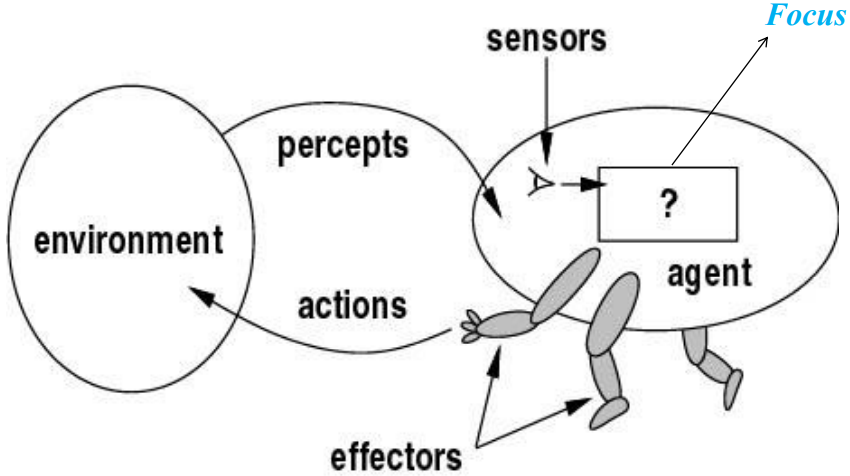
\includegraphics[scale=0.22]{Media/CicloPercezioneAzione.png}
                \caption{Ciclo percezione-azione}
            \end{figure}
            \subsection{Caratteristiche}
            \paragraph{} Gli \textbf{agenti}:
                \begin{itemize}
                    \item sono \textbf{situati}
                        \subitem ricevono percezioni da un ambiente
                        \subitem agiscono sull'ambiente mediante azioni (\textbf{attuatori})
                    \item hanno \textbf{abilita sociale}
                        \subitem sono capaci di comunicare, collaborare, difendersi da 
                        altri agenti
                    \item hanno \textbf{credenze, obiettivi, intenzioni, ...} 
                    \item sono \textbf{embodied}
                        \subitem hanno un \textbf{corpo}, fino a 
                        considerare i meccanismi delle \textbf{emozioni}
                \end{itemize}
            \subsection{Percezioni e azioni}
                \paragraph{} Una \textbf{percezione} è un input proveniente da sensori. La storia completa delle percezioni è detta \textbf{sequenza percettiva}.\\
                La \textbf{funzione agente} definisce l'\textbf{azione} da compiere per ogni sequenza percettiva (descrive completamente l'agente) ed è implementata attraverso un \textbf{programma agente}.
                \begin{figure}[htbp]
                    \centering
                    
\includegraphics[scale=0.5]{Media/FunzioneAgente.png}
                \end{figure}
                \begin{figure}[htbp]
                    \centering
                    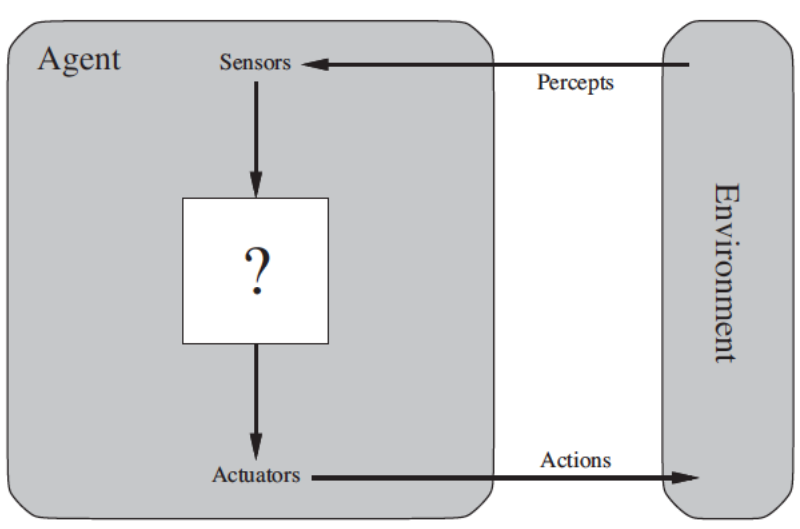
\includegraphics[scale=0.5]{Media/ArchitetturaAstrattaAgenteAmbiente.png}
                    \caption{Architettura astratta agente-ambiente}
                \end{figure}
                \begin{figure}[htbp]
                    \centering
                    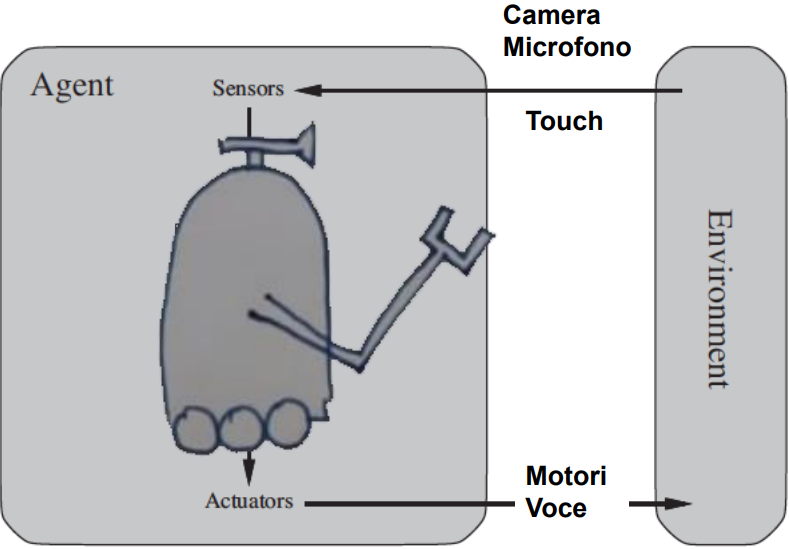
\includegraphics[scale=0.25]{Media/ArchitetturaRobot.png}
                    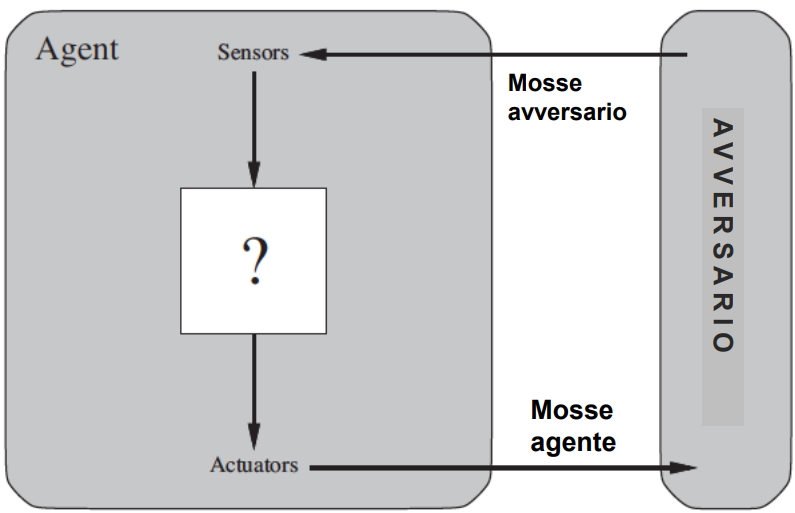
\includegraphics[scale=0.25]{Media/ArchitetturaGioco.png}
                    \caption{Esempi concreti di architettura agente-ambiente}
                \end{figure}
        \section{Agenti razionali}
            \paragraph{}Un \textbf{agente razionale} interagisce con il suo ambiente in maniera “efficace” (fa la cosa “giusta”).
            Serve un \textbf{criterio di valutazione oggettivo} dell’effetto delle azioni dell’agente (della sequenza di stati dell’ambiente).
            \paragraph{Definizione} L'\textbf{agente razionale} per ogni sequenza di percezioni compie l’azione che \textbf{massimizza il valore atteso} della 
            misura delle prestazioni, considerando le sue \textbf{percezioni passate} e la sua \textbf{conoscenza pregressa}.\\
            La razionalità è relativa e dipende da:
            \begin{itemize}
                \item la misura di prestazioni
                \item le conoscenze pregressa dell’ambiente 
                \item le percezioni presenti e passate (sequenza percettiva)
                \item le capacità dell’agente (azioni possibili)
            \end{itemize}
            \paragraph{Razionalità non onniscenza} Non si pretendono perfezione e conoscenza del futuro, ma \textbf{massimizzazione del risultato atteso},
            potrebbero essere necessarie azioni di acquisizioni di informazioni o esplorative.
            \paragraph{Razionalità e apprendimento} Raramente tutta la conoscenza sull'ambiente può essere fornita a priori dal programmatore.
            L’agente razionale deve essere in grado di \textbf{modificare il proprio comportamento con 
            l’esperienza} (le percezioni passate). Può migliorare esplorando, apprendendo, aumentando autonomia per operare in ambienti differenti o mutevoli.
        \section{Agenti autonomi}
            \paragraph{Definizione} L'\textbf{agente autonomo} è autonomo nella misura in cui il suo comportamento dipende dalla sua \textbf{capacità di ottenere esperienza}
            (non dall'aiuto del progettista). Un agente il cui comportamento fosse determinato solo dalla sua conoscenza built-in (pregressa), sarebbe non autonomo e poco flessibile.
\end{document}